\subsubsection{Human Tracking}
For human tracking and following, we implemented the TLD (Track-Learning Detection) algorithm\cite{kalal2012tracking}. TLD was proposed by Zdenek Kalal and is currently the state-of-art real time tracking algorithm. It combine the traditional tracking and detection algorithm so that it is more robust in consideration of distortion and partial occlusions. TLD algorithm consists of three modules as its name indicated. Tracking module estimate moving direction of the object according to the difference between two adjacent frames. Detection module detect the object in each frame independently. Learning module integrate the results of the tracking module and detection module to correct the detection errors and update the features of the target object.
We applied the TLD algorithm to human tracking and following tasks. Before the robot starts following, the human partner to be followed will be asked to stand in front of Kinect and the robot will record his/her features. When the instructor starts moving around, the robot will track and keep up with him. The robot also uses the depth information to keep away from the instructor at a safe distance.
Moverover, we use Kinect camera to analyze human skeleton and make simple analysis and judgment of body language. 
\subsubsection{Face Recognition}
For human-robot interaction, a robot is required to recognize different masters or guests in home service. We developed a face recognition system with two process: enrollment and recognition. During the enrollment process, a man is asked to stand in front of the RGB camera. A face detector based on haar feature from OpenCV is applied and the detected face will be stored. For a single person, the system stores 3-5 pictures.
We used face++ supported by Questyle Audio for face detection and implemented the face recognition algorithm based on sparse representation \cite{wright2009robust}. A redundant dictionary is trained offline using a set of training faces. The algorithm seeks the most sparse representation coefficient by solving a L1 optimization problem. The residual errors for different classes (persons) tell who is the unknown person: if the residual error for a specific class, for example, person A, is smaller than a specified threshold and the errors for other classes are larger than another specified threshold, the newcoming person is identified as person A. Fig.4 shows an example of the face recognition result. More details of this face recognition pipeline can be found in \cite{xia2015human}.
\begin{figure}[H]
	\centering
    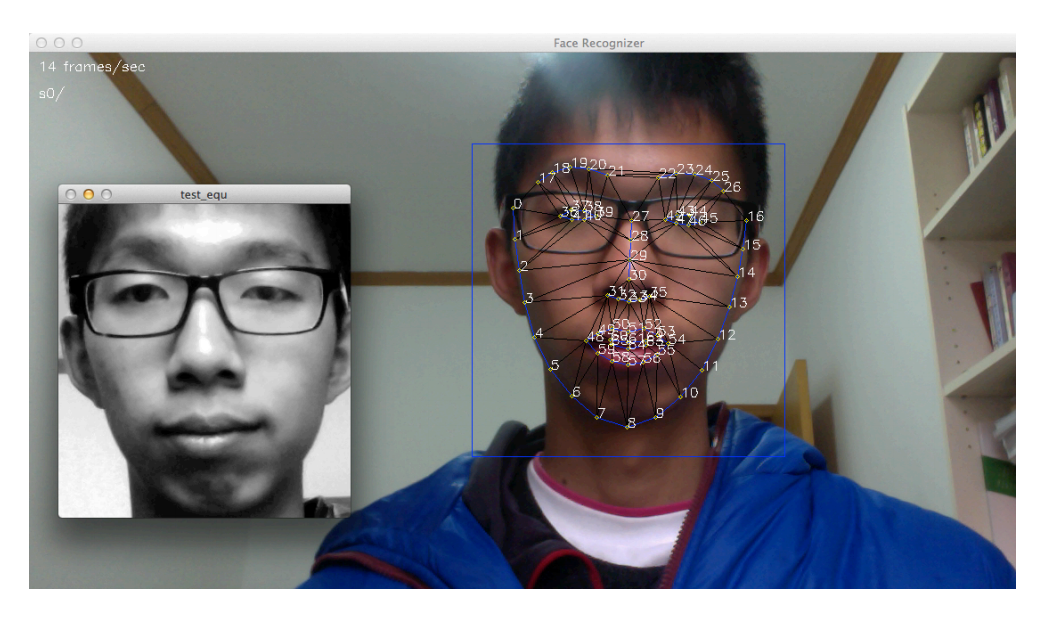
\includegraphics[scale=0.5]{face.png}
    \caption{face recognition}
\end{figure}
\subsubsection{Object recoginition}
\ 

Tinker uses a two-phase approach to recognize objects and precisely manipulate them. In the first phase, a point cloud is built from the Kinect depth camera to collect the features, and we use Fast Plane Extraction in Organized Point Clouds Using Agglomerative Hierarchical Clustering inside.
Real-time plane extraction in 3D point clouds
is crucial to many robotics applications. We present a novel
algorithm for reliably detecting multiple planes in real time in
organized point clouds obtained from devices such as Kinect
sensors. By uniformly dividing such a point cloud into non-
overlapping groups of points in the image space, we first
construct a graph whose node and edge represent a group of
points and their neighborhood respectively. We then perform
an agglomerative hierarchical clustering on this graph to sys-
tematically merge nodes belonging to the same plane until the
plane fitting mean squared error exceeds a threshold. Finally
we refine the extracted planes using pixel-wise region growing.
Our experiments demonstrate that the proposed algorithm can
reliably detect all major planes in the scene at a frame rate of
more than 35Hz for 640*480 point clouds, which to the best of
our knowledge is much faster than state-of-the-art algorithms.

For object classification, another image processing pipeline is implemented. We used fast YOLO \cite{1612.08242} for general object type detection. fast YOLO is a light-weight while precise nerual network for genral object detection and classification. Then we implemented a bag of words model \cite{csurka2004visual} to pair the object image with those collected in the library.
